\documentclass{jarticle}
\usepackage{amsmath,amssymb}
\usepackage{amsmath}
\usepackage[dvipdfmx]{graphicx}
\usepackage{here}
\usepackage{pifont}
\usepackage[left=2cm, right=2cm]{geometry}
\setcounter{MaxMatrixCols}{20}
\begin{document}
\section{結果}
$\mathcal{H}$を数値計算で対角化していく。
$N=1000$、$k_y$を横軸として変化させて縦軸に固有値をプロットし分散関係を描いた。結果は以下のようになった。\\
\begin{figure}[H]
	\centering
	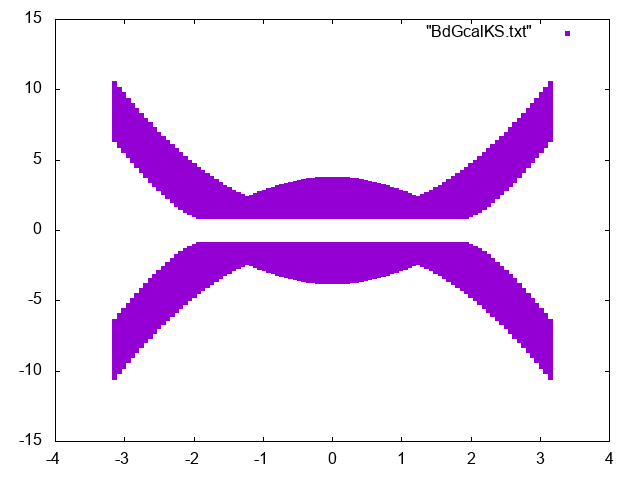
\includegraphics[scale=0.7]{BdGcalKSs.png}
	\caption{分散関係}
\end{figure}
次にグリーン関数を用いて状態密度を求める。
まずグリーン関数は
\begin{align}
G=(E+i\delta-H)^{-1}
\end{align}
であり、表面の状態密度は
\begin{align}
\rho=-\dfrac{1}{\pi}Im(G_{11}+G_{22})
\end{align}
で求められる。$E$を$-3$〜$3$で動かして$\rho$をプロットした。この時$\delta=10^{-3}$とした。
以下に結果を示す。
\begin{figure}[H]
	\centering
	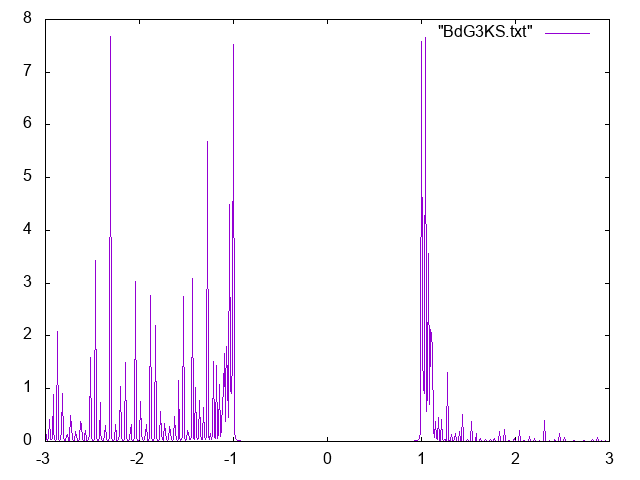
\includegraphics[scale=0.7]{BdG3KS1.png}
	\caption{状態密度}
\end{figure}
ここからエネルギーが$-1$〜$1$では状態がないことが分かる。
\end{document}